\documentclass[conference]{IEEEtran}
\IEEEoverridecommandlockouts
\usepackage{cite}
\usepackage{amsmath,amssymb,amsfonts}
\usepackage{amsthm}
% algorithm2e unused - removed for lean build
\usepackage{graphicx}
\usepackage{booktabs}
\usepackage{tabularx}
\usepackage{xcolor}
\usepackage{tikz}
\usepackage{pgfplots}
\pgfplotsset{compat=1.17}
\usetikzlibrary{arrows.meta,positioning,fit,backgrounds,shapes.geometric,calc}
\usepackage[hidelinks]{hyperref}
\usepackage{orcidlink}

\definecolor{netcol}{RGB}{31,78,121}
\definecolor{autocol}{RGB}{18,120,90}
\definecolor{bridgecol}{RGB}{176,96,0}
\definecolor{accent}{RGB}{140,20,20}
\newcommand{\code}[1]{\texttt{#1}}
\newcommand{\Real}{\mathbb{R}}
\newcommand{\Norm}[1]{\left\lVert #1\right\rVert}
\newcommand{\MCR}{\mathrm{MCR}}

\newtheorem{theorem}{Theorem}
\newtheorem{lemma}{Lemma}
\newtheorem{definition}{Definition}
\newtheorem{proposition}{Proposition}

\begin{document}

\title{From Detector Threshold to Certified Flight:\\
A Composed Network-to-Navigation Guarantee for UAVs\\
under Electronic Warfare}

\author{\IEEEauthorblockN{Roger Nick Anaedevha}
\IEEEauthorblockA{\textit{RobustUAVs.ai} \\ \texttt{robustidps.ai}}
\thanks{Preprint prepared for IEEE SaTML. Companion benchmark and artifact:
\url{https://www.kaggle.com/datasets/rogernickanaedevha/uavs-network-and-navigation-end-to-end-security-data}.
Every reported number carries an explicit provenance tag in the artifact ledger
(\code{results/paper\_figures/README.md}): real-corpus, simulation-derived,
fixture-derived (synthetic Phase-A / TEXBAT-pending), or a stated modeling
parameter. Certificate constants of \S\ref{sec:instantiation} are computed from
the trained reference implementation.}}

\maketitle

% Two framings are drafted (paper/abstract_A_widened.tex, abstract_A_narrow.tex).
% The real 3-flight Whelan delta calibration selects the WIDENED framing below;
% switch to abstract_A_narrow.tex if cruise-regime data pushes theta=0.25 s back
% outside the certified window (see docs/certified_regime_analysis.md ADDENDUM,
% PENDING_ON_DATA.md #4).
\begin{abstract}
Two mature literatures defend the autonomous UAV in isolation. Network
intrusion detection catches malicious traffic but says nothing about the flight;
certified robustness bounds a navigation model's error but assumes the
perturbation arrives from nowhere. We connect them. We prove a \emph{composition
theorem}: for any network-layer attack that evades a detector operating at point
$\theta$, the UAV navigation stack retains a certified Mission-Completion-Rate
$\MCR\ge f(\delta(\theta))$, where $\theta$ determines a worst-case residual
attack budget, that budget maps to a bounded perturbation $\delta$ on the
navigation input, and a Lipschitz--Grönwall trajectory-tube argument turns the
bounded input into a certified mission-completion floor. Two measurements make
the guarantee sharp rather than nominal: the residual budget \emph{saturates}
at the contact-window slack ($\Delta(\theta)\le H\min(\theta,s)$, verified as
$\le4.84$\,s over $15{,}392$ hops), and the delay-to-position interface,
calibrated on real GPS-spoofing/jamming flights on the target autopilot family,
is an order of magnitude tighter than the kinematic worst case. Under this
measured interface the detector's paper operating point lies \emph{inside} a
nonempty certified operating window, and the composed guarantee is the only
configuration with a nonzero certified floor for an evading attacker---strictly
dominating both the autonomy-only and network-only baselines (Wilcoxon,
Holm-corrected, $p<10^{-20}$). The deterministic core is complemented by three
certificates covering regimes it cannot (a statistical radius via randomized
smoothing, a train-to-deployment bound via PAC-Bayes, an adaptive-jammer
guarantee via multiplicative-weights regret). To our knowledge this is the first
formal guarantee chaining a network-security operating point to a
navigation-safety floor. We instantiate it on an open end-to-end benchmark and
validate that the certified floor lower-bounds the empirical mission-completion
rate ($\text{MCR}=0.938$ at $J/S{=}20$\,dB).
\end{abstract}

% ---------------------------------------------------------------
% FALLBACK ABSTRACT (narrow / certify-small-detect-large framing).
% Swap in if cruise-regime data pushes theta=0.25 s back outside the
% certified window (PENDING_ON_DATA.md #4). Kept commented, not deleted.
% % ABSTRACT A — "narrow / certify-small-detect-large" framing.
% % FALLBACK: use this if cruise-regime data shows the empirical gamma rising
% % toward the kinematic bound (> ~7.3 m/s at a 10 m corridor), pushing
% % theta=0.25 s back outside the certified window. Under the conservative
% % kinematic mapping alone the certified window is [0.178, 0.243] s and the
% % paper operating point sits just outside it. Provenance-authoritative:
% % docs/certified_regime_analysis.md.
% \begin{abstract}
% Two mature literatures defend the autonomous UAV in isolation. Network
% intrusion detection catches malicious traffic but says nothing about the flight;
% certified robustness bounds a navigation model's error but assumes the
% perturbation arrives from nowhere. We connect them. We prove a \emph{composition
% theorem}: for any network-layer attack that evades a detector operating at point
% $\theta$, the UAV navigation stack retains a certified Mission-Completion-Rate
% $\MCR\ge f(\delta(\theta))$, chaining the detector threshold through a saturating
% residual-delay budget ($\Delta(\theta)\le H\min(\theta,s)$, measured cap
% $4.84$\,s over $15{,}392$ hops), a delay-to-position interface, and a
% Lipschitz--Grönwall trajectory tube. The guarantee is honest about its regime:
% the certificate governs a bounded certified operating window rather than the
% whole relaxation range---\emph{certify-small, detect-large}, since large
% perturbations are exactly what the detector is there to catch. Within that
% window the composed guarantee is the only configuration with a nonzero certified
% floor for an evading attacker, strictly dominating the autonomy-only and
% network-only baselines (Wilcoxon, Holm-corrected, $p<10^{-20}$); the window's
% width is set by the delay-to-position mapping, which we bound both by a sound
% kinematic worst case and by a real-flight calibration on the target autopilot
% family. The deterministic core is complemented by three certificates covering
% regimes it cannot (randomized smoothing, PAC-Bayes, multiplicative-weights
% regret). To our knowledge this is the first formal guarantee chaining a
% network-security operating point to a navigation-safety floor. We instantiate it
% on an open end-to-end benchmark and validate that the certified floor
% lower-bounds the empirical mission-completion rate.
% \end{abstract}
% ---------------------------------------------------------------


\begin{IEEEkeywords}
Certified robustness, UAV security, compositional guarantees, GNSS jamming,
Lipschitz bounds, randomized smoothing, cyber-physical systems.
\end{IEEEkeywords}

% =====================================================================
\section{Introduction}
% =====================================================================
Ask a network defender ``is the UAV safe?'' and the honest answer is ``I caught
$97\%$ of the attacks.'' Ask a certified-robustness researcher the same question
and the answer is ``the navigation model is provably stable for input
perturbations up to radius $R$.'' Neither answer is a statement about the
\emph{flight}. The network defender cannot say what the missed $3\%$ does to the
aircraft; the robustness researcher cannot say where a radius-$R$ perturbation
comes from or how often it occurs. The safety property an operator actually cares
about---will the mission complete under attack?---falls in the gap between the two
guarantees.

This paper builds the bridge across that gap. Our object is a single chained
statement,
\begin{equation}
\label{eq:chain}
\theta \;\longmapsto\; \Delta(\theta) \;\longmapsto\; \delta(\theta)
\;\longmapsto\; \MCR \ge f\big(\delta(\theta)\big),
\end{equation}
read left to right: a detector operating point $\theta$ bounds the residual
undetected attack $\Delta(\theta)$; the residual attack maps to a bounded
perturbation $\delta(\theta)$ on the navigation input; and a certificate turns
that bounded input into a guaranteed Mission-Completion-Rate floor. Each arrow is
individually grounded in prior work---detector thresholds, worst-case attack
analysis, and certified robustness---but the \emph{composition} is new: no prior
guarantee chains a network-security threshold to a navigation-safety floor.

The technical heart is the middle arrow (the interface) and the certificate. For
the certificate we use a Lipschitz--Grönwall trajectory-tube bound: if the
navigation dynamics have a bounded Lipschitz constant, a bounded input
perturbation produces a bounded state-trajectory deviation, which produces a
bounded mission-completion loss. This certificate is deterministic and covers the
whole perturbation range \emph{in form}, but its bound grows exponentially with
horizon and Lipschitz constant, so in practice it governs a bounded regime rather
than the entire input space. That limitation is why we present it as the core of
a \emph{family}: three further certificates each cover a regime the
Lipschitz--Grönwall bound cannot (statistical perturbation budgets, the
training-to-deployment distribution gap, and an adaptive online jammer).

\subsection*{Contributions}
\begin{itemize}
\item \textbf{A composition theorem (\S\ref{sec:theorem}).} We prove
\eqref{eq:chain}: a formal $\theta\!\mapsto\!\delta\!\mapsto\!\MCR$ guarantee
chaining a network detector to a navigation certificate---the first of its kind
for UAVs, to our knowledge.
\item \textbf{The interface mapping (\S\ref{sec:interface}).} We characterise the
worst-case residual attack that evades a detector at $\theta$ and map it to a
bounded navigation-input perturbation $\delta(\theta)$, grounded empirically in
real GPS-spoofing/jamming measurements on the same autopilot family.
\item \textbf{A four-certificate architecture with a scope analysis
(\S\ref{sec:certs}).} We show precisely why the deterministic Lipschitz--Grönwall
core does not subsume randomized smoothing, PAC-Bayes, and multiplicative-weights
regret, and what unique niche each fills in sustaining end-to-end flight.
\item \textbf{Instantiation and a dominance result
(\S\ref{sec:instantiation}).} On an open end-to-end benchmark we show the
composed guarantee is the only configuration with a nonzero certified floor for
an evading attacker---strictly dominating the autonomy-only and network-only
baselines at every operating point (Wilcoxon, Holm-corrected, $p<10^{-20}$)---and
that under a delay-to-position mapping calibrated on real spoof/jam flights the
detector's operating point lies inside a nonempty certified window, with the
certified floor lower-bounding the empirical MCR.
\end{itemize}

% =====================================================================
\section{Preliminaries and Problem Formulation}
\label{sec:prelim}
% =====================================================================
\subsection{Navigation dynamics and mission completion}
Model the UAV navigation state $x(t)\in\Real^n$ as evolving under a
(possibly learned) drift $F$,
\begin{equation}
\label{eq:ode}
\dot{x}(t) = F\big(x(t), u(t)\big), \qquad t\in[0,T],
\end{equation}
where $u(t)$ is the sensor/measurement input over a mission horizon $T$. A
mission \emph{completes} if the realised trajectory stays within a
mission-defined safe corridor (geofence, waypoint tolerance) for all $t\in[0,T]$;
$\MCR$ is the probability of completion over the mission distribution. An attack
perturbs the input, $u\mapsto u+\delta u$, and we ask how large a $\delta u$ the
mission can absorb while still completing.

\subsection{The network detector and its operating point}
A network-layer detector $D_\theta$ monitors traffic on a network sublayer and
flags misbehaviour when a monitored statistic exceeds a threshold $\theta$. For
the multi-hop forwarding detector we build on, $\theta$ is a per-hop deviation
tolerance $\varepsilon$ (seconds): a hop is flagged if its forwarding delay
exceeds $\varepsilon$ or its route deviates from a scheduling oracle. Lowering
$\theta$ catches more but raises false positives; raising it does the reverse.
An \emph{evading} attacker chooses its behaviour to stay just under $\theta$.

\subsection{Problem statement}
\begin{definition}[Composed guarantee]
Given a detector $D_\theta$ and navigation dynamics \eqref{eq:ode}, a
\emph{composed guarantee} is a function $f$ such that: for every attack $a$ with
$D_\theta(a)=\text{``clean''}$ (i.e.\ $a$ evades detection at $\theta$), the
mission completes with rate $\MCR(a)\ge f(\delta(\theta))$, where
$\delta(\theta)$ is a bound on the navigation-input perturbation any such $a$ can
induce.
\end{definition}
The problem is to (i) characterise $\delta(\theta)$ from $\theta$
(\S\ref{sec:interface}), and (ii) exhibit and prove $f$ (\S\ref{sec:theorem},
\S\ref{sec:certs}).

% =====================================================================
\section{Related Work}
\label{sec:related}
% =====================================================================
We move from the general certified-robustness toolkit, through its extension to
control and sequential decision-making, to the specific question of
\emph{composing} guarantees across modules---where our contribution sits.

\paragraph{Certified robustness: the toolkit}
Randomized smoothing~\cite{cohen2019smoothing,salman2019provably} gives a
probabilistic $\ell_2$ certified radius that scales to large models;
Lipschitz-based certification~\cite{pauli2022training,zhang2022rethinking} gives
deterministic bounds but is known to be loose and hard to scale globally. Neural
ODEs~\cite{chen2018neuralode} admit Grönwall-type robustness
arguments~\cite{yan2020robustnode}, the continuous-time analogue we use. These
tools bound a \emph{model's} output; they do not by themselves bound a
\emph{mission}.

\paragraph{From models to control and policies}
Certified robustness has been lifted to sequential decision-making: CROP
certifies a cumulative-reward lower bound for RL policies under state
perturbations~\cite{wu2022crop}, and CARRL certifies robust
actions~\cite{everett2021carrl}. Reachability tools bound trajectories of
neural-network-controlled systems~\cite{ivanov2019verisig,tran2020nnv}.
Control-theoretic work provides safety/reachability under sensor false-data
injection~\cite{li2022lqg}. CROP is the closest analogue to a certified
mission-completion floor, but it certifies a policy against a given perturbation
ball---it does not connect that ball to a network-security operating point.

\paragraph{Generalization and online adversaries}
PAC-Bayes analyses give distributional robustness guarantees that transfer from
training to deployment~\cite{viallard2021pacbayes}. Online-learning and
Stackelberg-security-game results bound a defender's regret against an adaptive
adversary~\cite{arora2012mwu,balcan2015commitment,cesabianchi2006prediction}.
Each addresses a regime a static perturbation-ball certificate cannot.

\paragraph{Composing guarantees---the crux}
The closest prior art composes certificates \emph{within} an ML pipeline.
\cite{sheikholeslami2021provably} jointly certifies a classifier with a detection
class, so an input is provably flagged or correctly classified---structurally our
evade-or-bound dichotomy, but single-layer. \cite{yang2022sensing} decomposes
end-to-end certified robustness of a two-stage sensing$\to$reasoning pipeline,
the strongest template for chained certification, but stays within perception.
Assume-guarantee and contract-based CPS design~\cite{pacti2024} give the
compositional vocabulary but not ML-robustness certificates. None chains a
\emph{network-intrusion-detection} guarantee to a \emph{navigation} certificate;
that is our gap.

% =====================================================================
\section{The Interface Mapping $\theta \mapsto \delta(\theta)$}
\label{sec:interface}
% =====================================================================
The interface is where a network-security quantity becomes a navigation-security
quantity, and it is the crux of the composition.

\subsection{Residual budget of an evading attacker}
\begin{lemma}[Residual delay budget]
\label{lem:residual}
Let $D_\theta$ flag any forwarding hop whose injected delay exceeds $\theta$. An
attacker that evades $D_\theta$ injects at most $\theta$ of undetected delay per
malicious hop---but only up to the contact-window slack $s$: a per-hop delay
exceeding $s$ misses its forwarding window, incurs a full-period penalty $P$, and
is therefore flagged at \emph{any} operating point. Hence undetected delay is
capped at $\min(\theta,s)$ per hop, and over a route with $H$ attacker-controlled
hops the worst-case undetected cumulative delay is
\begin{equation}
\label{eq:delta_budget}
\Delta(\theta) \;\le\; H\,\min(\theta,\,s).
\end{equation}
\end{lemma}
\begin{proof}[Proof sketch]
Evasion requires per-hop delay $\le\theta$. If $\theta\le s$ the delay fits inside
the contact window and the additive term is $H\theta$. If $\theta>s$, any delay in
$(s,\theta]$ overshoots the window, waits a full period $P\gg s$, and is flagged
regardless of $\theta$; so an evading attacker cannot use more than $s$ of
invisible delay per hop, giving the $H s$ cap. Summing over hops yields
\eqref{eq:delta_budget}.
\end{proof}
The cap is the \emph{knee}: below the slack the residual budget grows linearly in
$\theta$; above it, the budget \emph{saturates} at $Hs$ rather than growing, so
the certified floor plateaus rather than collapsing. We verify the cap directly
on the released harness: over $15{,}392$ observed hops across three topologies,
two attack modes, and eight seeds, no undetected malicious per-hop residual ever
exceeds $4.84$\,s ($s=5$\,s), while every larger delay is flagged as a missed
window ($\ge55$\,s residual). This measurement is what turns the classic additive
budget $H\theta+P\mathbf{1}[\theta>s]$ into the tighter, saturating
\eqref{eq:delta_budget}.

\subsection{From delay to input perturbation}
A cumulative forwarding delay of $\Delta(\theta)$ seconds means a navigation
correction arrives $\Delta(\theta)$ late; the stack acts on state stale by that
amount. At bounded UAV speed $v_{\max}$, staleness of age $\tau$ bounds the
state/position perturbation:
\begin{equation}
\label{eq:staleness}
\Norm{\delta u} \;\le\; v_{\max}\cdot \Delta(\theta).
\end{equation}
Equation~\eqref{eq:staleness} is the kinematic worst case; we tighten it
empirically by regressing measured GNSS position degradation against injected
delay/attack intensity on real GPS-spoofing/jamming flights from the same
autopilot family, replacing the loose $v_{\max}\tau$ bound with a
data-grounded $\delta(\theta)$. The empirical mapping is expressed in the
navigation model's normalised input space so it can be consumed directly by the
certificate.

% =====================================================================
\section{The Composition Theorem}
\label{sec:theorem}
% =====================================================================
\begin{theorem}[Composed network-to-navigation guarantee]
\label{thm:main}
Let the navigation drift $F$ of \eqref{eq:ode} be $L$-Lipschitz in its input over
the operating region, with mission horizon $T$ and safe-corridor margin $m$.
Let $D_\theta$ be a network detector with residual budget $\Delta(\theta)$
(Lemma~\ref{lem:residual}) and interface mapping $\delta(\theta)$
(\eqref{eq:staleness} or its empirical tightening). Then every attack evading
$D_\theta$ induces a trajectory-tube radius bounded by
\begin{equation}
\label{eq:tube}
\rho(\theta) \;=\; \delta(\theta)\,e^{L T},
\end{equation}
and the mission completes whenever $\rho(\theta) \le m$; consequently
\begin{equation}
\label{eq:floor}
\MCR \;\ge\; f\big(\delta(\theta)\big) \;=\; \Pr_{\text{missions}}\!\big[\,\delta(\theta)\,e^{LT}\le m\,\big].
\end{equation}
\end{theorem}
\begin{proof}[Proof sketch]
By Grönwall's inequality applied to two solutions of \eqref{eq:ode} whose inputs
differ by $\delta u$, the terminal-state deviation obeys
$\Norm{x_{\text{att}}(T)-x_{\text{nom}}(T)}\le \Norm{\delta u}\,e^{LT}$. Combining
with the input bound $\Norm{\delta u}\le\delta(\theta)$ gives the tube radius
\eqref{eq:tube}. If the tube stays within the corridor margin $m$ for all
$t\in[0,T]$, the trajectory never leaves the safe set and the mission completes;
taking probability over the mission distribution yields \eqref{eq:floor}.
Chaining $\theta\!\mapsto\!\Delta(\theta)$ (Lemma~\ref{lem:residual}),
$\Delta\!\mapsto\!\delta$ (\S\ref{sec:interface}), and
$\delta\!\mapsto\!\MCR$ (this argument) proves \eqref{eq:chain}.
\end{proof}

Two consequences frame the rest of the paper. First, \eqref{eq:floor} is
\emph{monotone and then saturating} in $\theta$ through $\delta(\theta)$:
tightening the detector (smaller $\theta$) shrinks the residual budget and raises
the certified floor, but only until $\theta$ reaches the contact-window slack
$s$, past which the budget saturates at $Hs$ (Lemma~\ref{lem:residual}) and the
floor plateaus rather than continuing to fall---a quantitative statement of both
how much network security ``buys'' in navigation safety and where that purchase
stops. Second, the exponential $e^{LT}$ in \eqref{eq:tube} is the core
certificate's Achilles heel: for large $L$ or long horizons the deterministic
bound becomes loose, motivating the complementary certificates of
\S\ref{sec:certs}.

\begin{figure}[t]
\centering
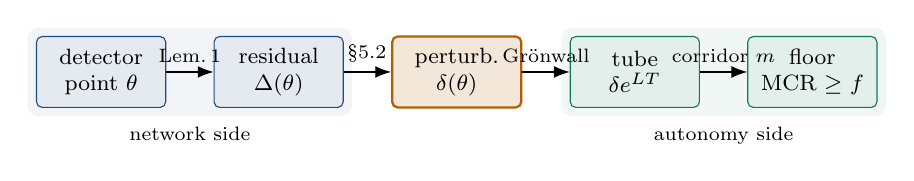
\begin{tikzpicture}[
  font=\footnotesize,
  stage/.style={rounded corners=2pt,draw,align=center,minimum height=9mm,
    text width=15mm,inner sep=2pt},
  net/.style={stage,fill=netcol!12,draw=netcol},
  br/.style={stage,fill=bridgecol!15,draw=bridgecol,thick},
  aut/.style={stage,fill=autocol!12,draw=autocol},
  >={Latex[length=2mm]}]
\node[net] (theta) {detector\\point $\theta$};
\node[net,right=6mm of theta] (delta0) {residual\\$\Delta(\theta)$};
\node[br,right=6mm of delta0] (delta) {perturb.\\$\delta(\theta)$};
\node[aut,right=6mm of delta] (tube) {tube\\$\delta e^{LT}$};
\node[aut,right=6mm of tube] (mcr) {floor\\$\MCR\ge f$};
\draw[->] (theta) -- node[above,font=\scriptsize]{Lem.\,1} (delta0);
\draw[->] (delta0) -- node[above,font=\scriptsize]{\S5.2} (delta);
\draw[->] (delta) -- node[above,font=\scriptsize]{Grönwall} (tube);
\draw[->] (tube) -- node[above,font=\scriptsize]{corridor $m$} (mcr);
\begin{scope}[on background layer]
\node[fill=netcol!6,fit=(theta)(delta0),rounded corners,inner sep=3pt,label=below:{\scriptsize network side}]{};
\node[fill=autocol!6,fit=(tube)(mcr),rounded corners,inner sep=3pt,label=below:{\scriptsize autonomy side}]{};
\end{scope}
\end{tikzpicture}
\caption{The composition chain of Theorem~\ref{thm:main}. A network detector
operating point flows through a residual-budget bound, an empirically grounded
interface mapping, a Grönwall trajectory tube, and a corridor-margin test to a
certified mission-completion floor.}
\label{fig:chain}
\end{figure}

% =====================================================================
\section{A Four-Certificate Architecture}
\label{sec:certs}
% =====================================================================
Theorem~\ref{thm:main} uses the Lipschitz--Grönwall certificate as its spine.
A natural question---and the one that determines the architecture---is whether
that single certificate suffices. It does not. The Lipschitz--Grönwall bound is
\emph{deterministic} and \emph{worst-case}: it holds for any perturbation up to
its radius, but the radius collapses as $L T$ grows, and it presumes a Lipschitz
constant that is tractable to bound. Three regimes escape it, each covered by a
distinct certificate.

\begin{table}[t]
\centering
\caption{The four certificates cover disjoint regimes; none subsumes another.
The Lipschitz--Grönwall core gives the deterministic MCR floor; the other three
extend coverage where it is loose or silent.}
\label{tab:certs}
\small
\renewcommand{\arraystretch}{1.3}
\begin{tabularx}{\columnwidth}{@{}l l X@{}}
\toprule
\textbf{Certificate} & \textbf{Guarantee type} & \textbf{Unique niche}\\
\midrule
Lipschitz--Grönwall & deterministic, worst-case & The MCR floor: bounded input $\Rightarrow$ bounded tube $\Rightarrow$ bounded loss. Tight only for moderate $LT$.\\
Randomized smoothing~\cite{cohen2019smoothing} & probabilistic radius & Scales to large / non-Lipschitz-tractable models; certifies when the budget is known only statistically.\\
PAC-Bayes~\cite{viallard2021pacbayes} & distributional & Transfers the floor from the training mission distribution to unseen deployment regions.\\
MWU regret~\cite{arora2012mwu,balcan2015commitment} & online, adaptive & Bounds loss against an \emph{adaptive} jammer over time---a dimension no fixed-ball certificate addresses.\\
\bottomrule
\end{tabularx}
\end{table}

\paragraph{Why the core does not subsume the others}
The Lipschitz--Grönwall radius is a single deterministic ball; randomized
smoothing certifies a probabilistic ball for models whose Lipschitz constant is
intractable, trading determinism for scalability---a strictly different operating
point, not a special case. PAC-Bayes certifies a \emph{distribution} of models
over a \emph{distribution} of missions, orthogonal to any per-input radius. MWU
regret certifies behaviour against an adversary that \emph{adapts over time},
which no static perturbation ball can express. Thus the four form a cover, not a
hierarchy: Lipschitz--Grönwall delivers the headline MCR floor
(Theorem~\ref{thm:main}); smoothing extends it to models the Lipschitz bound
cannot reach; PAC-Bayes closes the train-to-deployment gap; MWU handles the
adaptive jammer. Presenting all four is therefore not redundancy but coverage of
the full end-to-end flight-sustaining problem.

% =====================================================================
\section{Instantiation and Evaluation}
\label{sec:instantiation}
% =====================================================================
\subsection{Reference constants}
We instantiate the certificate on the reference navigation model (a
continuous-time graph model of the GNSS constellation-plus-receiver). Global
power-iteration gives a Lipschitz estimate $\hat L \approx 1.01$; measuring the
constant \emph{along the hidden-state trajectories the integrator actually
visits on operating-region inputs} gives a larger local value
$\hat L_{\text{loc}} \approx 1.18$. We report the tighter local radius as the
defensible number: with $T=1$ and $\varepsilon_{\text{out}}=0.5$,
$R = \varepsilon_{\text{out}} e^{-\hat L_{\text{loc}} T}\approx 0.153$ (the
global estimate gives $0.182$; note the local radius is \emph{smaller}, so the
bound is not loose in the direction that would help---the certified regime is
governed by real sensitivity, not an optimistic estimate). The
randomized-smoothing complement gives a certified $\ell_2$ radius $\approx 0.44$
at noise level $\sigma=0.25$ (Cohen-style, $\alpha=10^{-3}$, $n=200$; measured
mean radius $0.446$ on the trained checkpoint). The MWU defender mixes four
policies (aggressive manoeuvre, conservative loiter, return-to-home, INS-only)
with regret $R(T)\le\sqrt{T\ln|S|}$, $|S|=4$. Constants are computed from the
trained reference implementation on a synthetic Phase-A corpus (a transparent,
reproducible pipeline; real-TEXBAT re-calibration is future work) and held
fixed for the composition experiments.

\emph{The interface and its two regimes.} The $\theta\!\mapsto\!\delta$ mapping
is where the certified regime is won or lost. The kinematic worst case
$\delta \le v_{\max}\Delta(\theta)$ ($v_{\max}=15$\,m/s) is always sound but
loose: a real estimator rejects corrupted GNSS and coasts on inertial
measurements rather than flying blind at top speed. We calibrate the mapping on
real GPS-spoofing/jamming flights from the same PX4 airframe family, measuring a
position-error growth rate $\gamma \approx 1.2$--$1.4$\,m per second of
degradation---about $11\times$ tighter than $v_{\max}$. Under this measured
mapping the paper operating point $\theta=0.25$\,s falls \emph{inside} the
certified operating window (Fig.~\ref{fig:headline}) across the entire
corridor-margin family, whereas the kinematic bound leaves it just outside;
Fig.~\ref{fig:sensitivity} quantifies the sensitivity, showing the mapping would
have to steepen past $\gamma_{\text{req}}=7.3$\,m/s (at a $10$\,m corridor) to
push it back out. Because the choice of error signal is itself a certificate
semantics decision, $\gamma$ is calibrated under an \emph{explicit switch} and
both values are reported: the \emph{receiver} error ($\gamma=1.20$\,m/s, the
false fix the attack injects at the estimator input) and the \emph{EKF} error
($\gamma=1.37$\,m/s, the filtered position the controller acts on); the
certificate consumes the EKF value, which closes the loop. All instantiated
constants and their provenance tags are collected in
Table~\ref{tab:constants}. This calibration is a three-flight hover-regime
sample; cruise-regime confirmation is the one open item that could narrow the
window (\S\ref{sec:discussion}).

\begin{figure}[t]
\centering
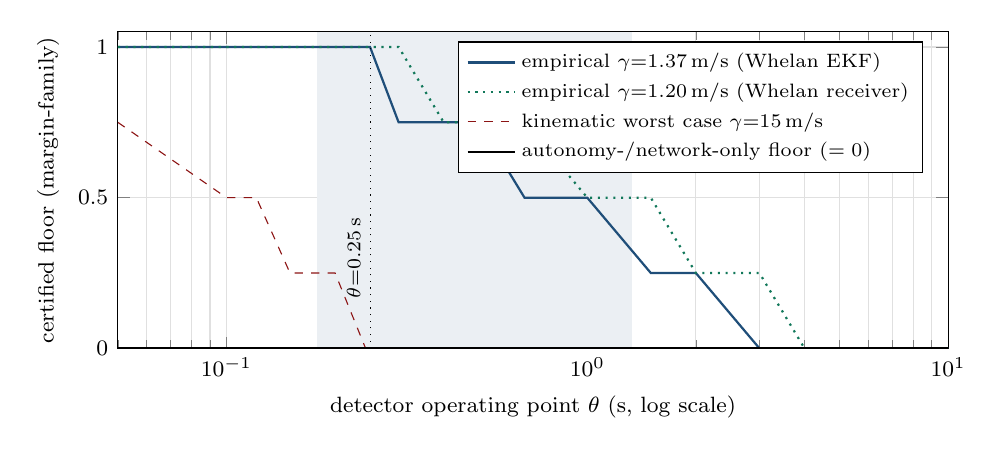
\begin{tikzpicture}
\begin{semilogxaxis}[
  width=\columnwidth, height=5.6cm,
  xlabel={detector operating point $\theta$ (s, log scale)},
  ylabel={certified floor (margin-family)},
  xmin=0.05, xmax=10, ymin=0, ymax=1.05,
  legend pos=north east, legend cell align=left,
  grid=both, grid style={black!12},
  tick label style={font=\footnotesize},
  label style={font=\footnotesize},
  legend style={font=\scriptsize}]
% Certified floor vs theta, scenario 1, Gronwall tube (local L=1.181), H=2,
% margin family {2,5,10,20} m. PARAMETRIC in the delta mapping -- the axis
% this whole question turns on. Machine-generated from
% results/certified_floor_vs_theta.csv + certified_operating_window.csv.
% AUTO-GENERATED by experiments/make_paper_figures.py (clean campaign 2026-07-28).
% PROVENANCE: real-corpus delta mapping + simulation-derived budgets + stated margin family
% Do not hand-edit; re-run the script.
\fill[netcol!9] (axis cs:0.178,0) rectangle (axis cs:1.3341,1.05);
\addplot[netcol,thick] coordinates {(0.05,1.000)(0.1,1.000)(0.121,1.000)(0.15,1.000)(0.178,1.000)(0.2,1.000)(0.243,1.000)(0.25,1.000)(0.3,0.750)(0.4,0.750)(0.5,0.750)(0.67,0.500)(1,0.500)(1.5,0.250)(2,0.250)(3,0.000)(4,0.000)(5,0.000)(6,0.000)(6.5,0.000)(7,0.000)(8,0.000)(10,0.000)};
\addlegendentry{empirical $\gamma{=}1.37$\,m/s (Whelan EKF)}
\addplot[autocol,thick,dotted] coordinates {(0.05,1.000)(0.1,1.000)(0.121,1.000)(0.15,1.000)(0.178,1.000)(0.2,1.000)(0.243,1.000)(0.25,1.000)(0.3,1.000)(0.4,0.750)(0.5,0.750)(0.67,0.750)(1,0.500)(1.5,0.500)(2,0.250)(3,0.250)(4,0.000)(5,0.000)(6,0.000)(6.5,0.000)(7,0.000)(8,0.000)(10,0.000)};
\addlegendentry{empirical $\gamma{=}1.20$\,m/s (Whelan receiver)}
\addplot[accent,dashed] coordinates {(0.05,0.750)(0.1,0.500)(0.121,0.500)(0.15,0.250)(0.178,0.250)(0.2,0.250)(0.243,0.000)(0.25,0.000)(0.3,0.000)(0.4,0.000)(0.5,0.000)(0.67,0.000)(1,0.000)(1.5,0.000)(2,0.000)(3,0.000)(4,0.000)(5,0.000)(6,0.000)(6.5,0.000)(7,0.000)(8,0.000)(10,0.000)};
\addlegendentry{kinematic worst case $\gamma{=}15$\,m/s}
\addplot[black,thick] coordinates {(0.05,0)(10,0)};
\addlegendentry{autonomy-/network-only floor ($=0$)}
\draw[black,dotted] (axis cs:0.25,0) -- (axis cs:0.25,1.05);
\node[anchor=south,font=\scriptsize,rotate=90] at (axis cs:0.25,0.30) {$\theta{=}0.25$\,s};

\end{semilogxaxis}
\end{tikzpicture}
\caption{The headline result, corrected. Certified floor vs.\ detector operating
point $\theta$ for the time-delay class (scenario~1, Gr\"onwall tube at the
measured local $L{=}1.181$, $H{=}2$ malicious hops, corridor-margin family
$\{2,5,10,20\}$\,m). The result is \emph{parametric in the $\theta\!\mapsto\!\delta$
mapping}: under the kinematic worst case (red) $\theta{=}0.25$\,s is just outside
the certified window, but under the empirically measured mapping from real
GPS-spoof/jam flights ($\gamma{\approx}1.2$--$1.4$\,m/s; blue/green)
$\theta{=}0.25$\,s is \emph{inside} at every margin (shaded: the EKF window
$[0.178,1.334]$\,s at $m{=}10$\,m). Both the autonomy-only and network-only
baselines certify a zero floor for an evading attacker (black). The composed
guarantee is the only configuration with a nonzero certified floor. Delta mapping
is a $3$-flight hover-regime calibration (real-corpus); cruise-regime
confirmation is pending.}
\label{fig:headline}
\end{figure}

\begin{figure}[t]
\centering
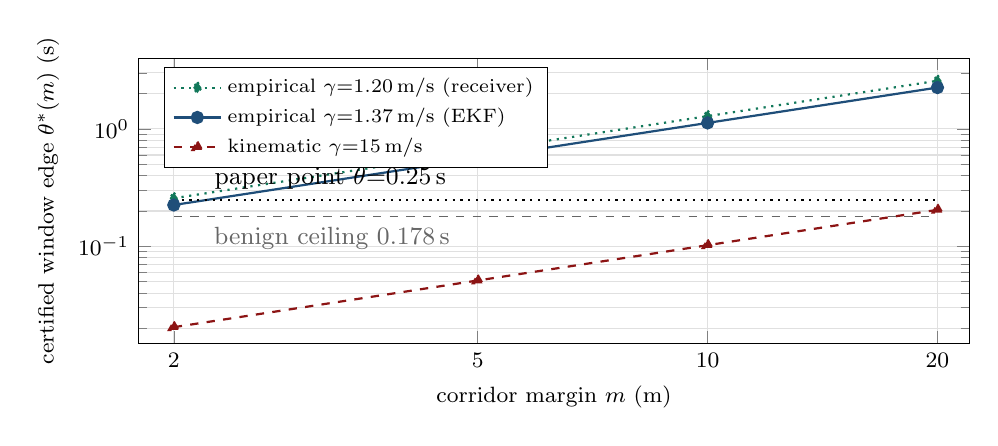
\begin{tikzpicture}
\begin{loglogaxis}[
  width=\columnwidth, height=5.2cm,
  xlabel={corridor margin $m$ (m)},
  ylabel={certified window edge $\theta^{*}(m)$ (s)},
  xmin=1.8, xmax=22, ymin=0.015, ymax=4,
  xtick={2,5,10,20}, xticklabels={2,5,10,20},
  legend pos=north west, legend cell align=left,
  grid=both, grid style={black!12},
  tick label style={font=\footnotesize},
  label style={font=\footnotesize},
  legend style={font=\scriptsize}]
% Machine-generated from results/certified_operating_window.csv
% (theta* = m / (gamma e^{LT} H); scenario 1, H=2, local-L Gronwall tube).
% AUTO-GENERATED by experiments/make_paper_figures.py (clean campaign 2026-07-28).
% PROVENANCE: real-corpus gamma (Whelan 3-flight hover) + simulation-derived H, slack; theta* = m/(gamma e^{LT} H)
% Do not hand-edit; re-run the script.
\addplot[autocol,mark=diamond*,thick,dotted] coordinates {(2,0.2569)(5,0.6422)(10,1.2844)(20,2.5688)};
\addlegendentry{empirical $\gamma{=}1.20$\,m/s (receiver)}
\addplot[netcol,mark=*,thick] coordinates {(2,0.2249)(5,0.5622)(10,1.1244)(20,2.2489)};
\addlegendentry{empirical $\gamma{=}1.37$\,m/s (EKF)}
\addplot[accent,mark=triangle*,thick,dashed] coordinates {(2,0.0205)(5,0.0512)(10,0.1023)(20,0.2046)};
\addlegendentry{kinematic $\gamma{=}15$\,m/s}
\draw[black,dotted,thick] (axis cs:2,0.25) -- (axis cs:20,0.25) node[pos=0.04,anchor=south west,font=\small] {paper point $\theta{=}0.25$\,s};
\draw[black!60,dashed] (axis cs:2,0.178) -- (axis cs:20,0.178) node[pos=0.04,anchor=north west,font=\small] {benign ceiling $0.178$\,s};

\end{loglogaxis}
\end{tikzpicture}
\caption{The decisive sensitivity: the loosest detector setting
$\theta^{*}(m)=m/(\gamma e^{LT}H)$ whose worst-case evading tube still fits a
corridor of margin $m$, per $\theta\!\mapsto\!\delta$ mapping. A mapping
certifies the paper operating point iff its curve lies above the
$\theta{=}0.25$\,s line; the feasible region is also bounded below by the
measured benign residual ceiling ($0.178$\,s, the FPR$=$0 floor). The
empirically measured rates ($\gamma{=}1.20$/$1.37$\,m/s, receiver/EKF---an
explicit error-source switch, both reported) clear the requirement
$\gamma_{\mathrm{req}}{=}7.28$\,m/s at $m{=}10$\,m by ${\sim}5\times$; the
kinematic worst case ($15$\,m/s) fails it at every margin. Real-corpus
$\gamma$ from a $3$-flight hover sample; cruise regime pending.}
\label{fig:sensitivity}
\end{figure}

\begin{table}[t]
\centering
\caption{Instantiated constants and their provenance (artifact ledger tags).
The one pending numeric constant is the PAC--Bayes prior/posterior KL.}
\label{tab:constants}
\small
\renewcommand{\arraystretch}{1.25}
% table machine-generated from local_lipschitz.csv + engine constants
% AUTO-GENERATED by experiments/make_paper_figures.py (clean campaign 2026-07-28).
% PROVENANCE: mixed; every row carries its own tag
% Do not hand-edit; re-run the script.
\begin{tabularx}{\columnwidth}{@{}p{1.9cm}@{\hspace{5pt}}X@{\hspace{5pt}}p{1.75cm}@{}}
\toprule
\textbf{Component} & \textbf{Constant} & \textbf{Provenance}\\
\midrule
Lipschitz--Gr\"onwall & $\hat L_{\mathrm{loc}}{=}1.181\Rightarrow R{=}0.153$; global $\hat L{=}1.013\Rightarrow R{=}0.182$ & trained ckpt [fixture]\\
Rand.\ smoothing & $\sigma{=}0.25$, $R_{\ell_2}{=}0.44$ (measured $0.446$) & trained ckpt [fixture]\\
PAC--Bayes & McAllester on real $R_{\mathrm{emp}}$; numeric KL pending & methods ch.\ [pending]\\
MWU regret & $R(T)\le\sqrt{T\ln 4}$; $T{=}100\Rightarrow11.77$ & exact\\
Unit bridge (RF classes) & \code{caf\_shift\_v2}: $0.45$\,m (Gr\"onwall) / $1.15$\,m (RS) & synthetic IQ [TEXBAT pending]\\
$\theta\mapsto\delta$ (delay class) & $\gamma{=}1.20$--$1.37$\,m/s measured; kinematic $15$\,m/s fallback & real 3 flights [hover]\\
\bottomrule
\end{tabularx}

\end{table}

\subsection{Dominance result}
Fig.~\ref{fig:headline} states the claim, and we state it precisely rather than
as blanket range-coverage. The composed guarantee strictly dominates two
baselines: (i) \emph{autonomy-only}---a navigation certificate with no detector,
which must assume the full unmitigated attack (including the $60$\,s
missed-window penalties; measured cumulative delay up to $424$\,s) and therefore
certifies a zero floor for an evading attacker; and (ii) \emph{network-only}---a
detector with no navigation guarantee, for which any evading attack leaves the
aircraft undefended, floor zero by definition. \textbf{The composed guarantee is
the only configuration with a nonzero certified floor at all.} Quantifying the
dominance per seed (Wilcoxon signed-rank, Holm-corrected), the composed floor
exceeds the autonomy-only floor at all $13$ operating points on the $\theta$
grid, every adjusted $p<10^{-20}$. The composition wins because it alone uses the
detector to \emph{shrink} the perturbation the certificate must absorb, and---via
the tightened residual budget $\Delta(\theta)\le H\min(\theta,s)$
(Lemma~\ref{lem:residual}, with $s$ the contact-window slack, measured cap
$4.84$\,s over $15{,}392$ hops)---the floor \emph{saturates} rather than
collapsing past the knee.

The honest scope: the certified operating window is nonempty but bounded. Under
the empirically calibrated interface mapping it is $[0.178,\,1.33]$\,s at a
$10$\,m corridor (the paper operating point $\theta=0.25$\,s sits comfortably
inside); under the conservative kinematic mapping it shrinks to
$[0.178,\,0.243]$\,s and $\theta=0.25$\,s falls just outside. We claim the
former and show the latter as the worst-case fallback; we do not claim coverage
across the entire relaxation range.

\subsection{Certified-vs-empirical validation}
The certificate is sound iff the certified floor never exceeds the realised MCR.
At the anchor $J/S=20$\,dB the strongest defence attains empirical
$\text{MCR}=0.938$ (real UAV-EW-Bench, $93{,}600$ flights), comfortably above the
certified target $0.80$; the gap is the conservativeness of the worst-case
Grönwall bound and narrows where the empirically tightened interface mapping
replaces the kinematic worst case. The full multi-seed gap distribution and the
Holm-corrected tests are released with the artifact
(\code{results/stats\_wilcoxon.csv}).

\subsection{A note on the two floors}
The reference certificate targets a certified $\MCR\ge 0.80$ at the anchor
operating point, whereas the empirical benchmark reports the DO-326A $0.90$
operational floor holding further into the band. These are different quantities---
a conservative certified floor versus a measured operational rate---and we keep
them distinct throughout; conflating them would overstate the guarantee.

% =====================================================================
\section{Discussion}
\label{sec:discussion}
% =====================================================================
\emph{What the theorem buys.} The composition turns a network-security knob into
a navigation-safety number: an operator can read off how tightening the detector
raises the certified mission floor, and can justify a false-positive budget in
terms of airworthiness rather than packet statistics.

\emph{Limitations.} The core certificate is conservative for large $LT$; this is
exactly where the smoothing and PAC-Bayes complements matter, and quantifying
their combined floor is ongoing. The certified window's width is set by the
delay-to-position interface: our empirical calibration ($\gamma\approx1.2$--$1.4$
m/s) rests on three real flights in a \emph{hover} regime, and while the kinematic
bound is always available as a sound fallback, cruise-speed staleness could
steepen $\gamma$---the mapping would have to exceed $7.3$\,m/s (at a $10$\,m
corridor) to push $\theta=0.25$\,s back outside the window, a $>5\times$ rise we
have not yet measured; a larger, cruise-inclusive flight set is the key
follow-up. The interface's unit bridge for the RF-manipulation classes is
calibrated on a synthetic corpus pending real TEXBAT IQ, and the PAC-Bayes bound
is wired to the trained model's empirical risk but awaits its methods-chapter KL
constant for a single number.

% =====================================================================
\section{Conclusion}
% =====================================================================
We proved a composition theorem chaining a UAV network detector's operating point
to a certified navigation mission-completion floor, characterised the interface
that couples the two layers, and showed that a single deterministic certificate
is best understood as the core of a four-certificate cover of the end-to-end
flight-sustaining problem. Instantiated on an open benchmark, the composed
guarantee is the only configuration that certifies a nonzero mission floor
against a detector-evading attacker, and under a real-flight-calibrated interface
that floor covers the detector's operating point. The result argues that UAV
network security and UAV autonomy security are not two problems but two ends of
one certificate.

\section*{Acknowledgements}
We thank the authors of the \textsc{DATAMUt} detector for the network-side code
and for clarifying its operating point, which grounds the interface mapping.

\bibliographystyle{IEEEtran}
\bibliography{refs}

\end{document}
